% Created by tikzDevice version 0.10.1 on 2018-01-24 12:32:35
% !TEX encoding = UTF-8 Unicode
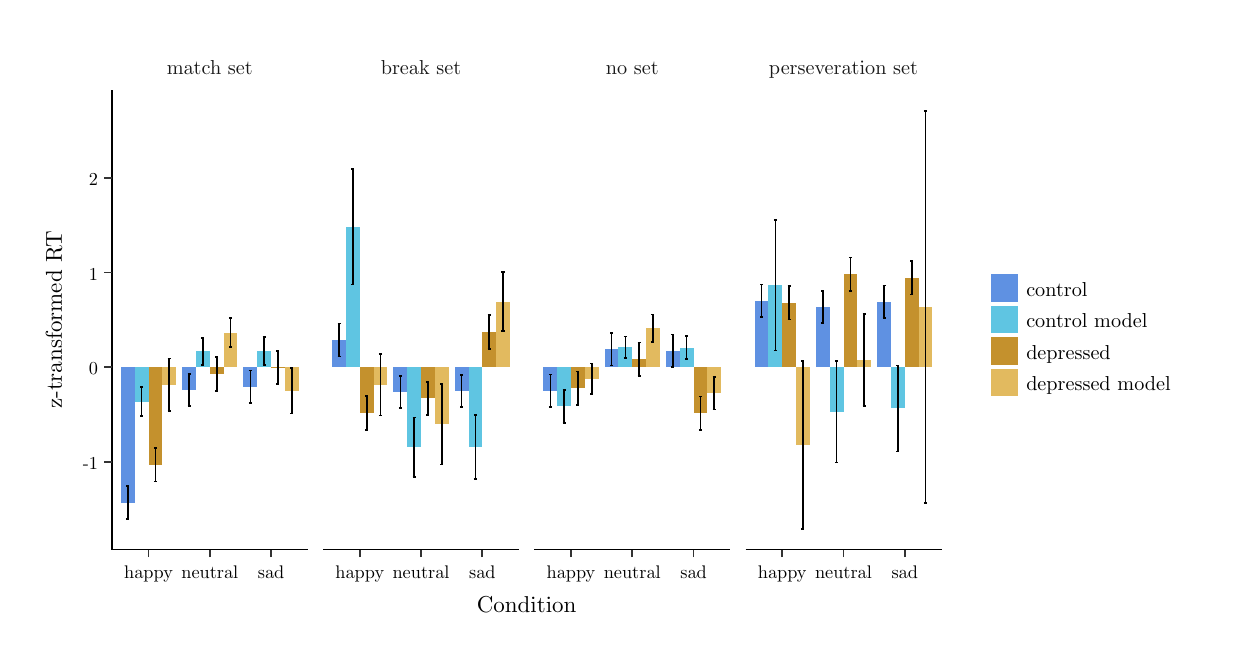
\begin{tikzpicture}[x=1pt,y=1pt]
\definecolor{fillColor}{RGB}{255,255,255}
\path[use as bounding box,fill=fillColor,fill opacity=0.00] (0,0) rectangle (433.62,216.81);
\begin{scope}
\path[clip] (  0.00,  0.00) rectangle (433.62,216.81);
\definecolor{drawColor}{RGB}{255,255,255}
\definecolor{fillColor}{RGB}{255,255,255}

\path[draw=drawColor,line width= 0.6pt,line join=round,line cap=round,fill=fillColor] (  0.00,  0.00) rectangle (433.62,216.81);
\end{scope}
\begin{scope}
\path[clip] ( 30.40, 28.22) rectangle (101.23,194.25);
\definecolor{fillColor}{RGB}{255,255,255}

\path[fill=fillColor] ( 30.40, 28.22) rectangle (101.23,194.25);
\definecolor{fillColor}{RGB}{226,186,95}

\path[fill=fillColor] ( 48.66, 87.75) rectangle ( 53.64, 94.12);
\definecolor{fillColor}{RGB}{196,145,45}

\path[fill=fillColor] ( 43.68, 58.86) rectangle ( 48.66, 94.12);
\definecolor{fillColor}{RGB}{95,197,226}

\path[fill=fillColor] ( 38.70, 81.69) rectangle ( 43.68, 94.12);
\definecolor{fillColor}{RGB}{95,145,226}

\path[fill=fillColor] ( 33.72, 45.23) rectangle ( 38.70, 94.12);
\definecolor{fillColor}{RGB}{226,186,95}

\path[fill=fillColor] ( 70.79, 94.12) rectangle ( 75.77,106.65);
\definecolor{fillColor}{RGB}{196,145,45}

\path[fill=fillColor] ( 65.81, 91.63) rectangle ( 70.79, 94.12);
\definecolor{fillColor}{RGB}{95,197,226}

\path[fill=fillColor] ( 60.83, 94.12) rectangle ( 65.81, 99.82);
\definecolor{fillColor}{RGB}{95,145,226}

\path[fill=fillColor] ( 55.85, 85.93) rectangle ( 60.83, 94.12);
\definecolor{fillColor}{RGB}{226,186,95}

\path[fill=fillColor] ( 92.93, 85.61) rectangle ( 97.91, 94.12);
\definecolor{fillColor}{RGB}{196,145,45}

\path[fill=fillColor] ( 87.95, 94.00) rectangle ( 92.93, 94.12);
\definecolor{fillColor}{RGB}{95,197,226}

\path[fill=fillColor] ( 82.96, 94.12) rectangle ( 87.95,100.03);
\definecolor{fillColor}{RGB}{95,145,226}

\path[fill=fillColor] ( 77.98, 87.05) rectangle ( 82.96, 94.12);
\definecolor{drawColor}{RGB}{0,0,0}

\path[draw=drawColor,line width= 0.6pt,line join=round] ( 50.59, 97.30) --
	( 51.70, 97.30);

\path[draw=drawColor,line width= 0.6pt,line join=round] ( 51.15, 97.30) --
	( 51.15, 78.20);

\path[draw=drawColor,line width= 0.6pt,line join=round] ( 50.59, 78.20) --
	( 51.70, 78.20);

\path[draw=drawColor,line width= 0.6pt,line join=round] ( 45.61, 64.92) --
	( 46.72, 64.92);

\path[draw=drawColor,line width= 0.6pt,line join=round] ( 46.17, 64.92) --
	( 46.17, 52.81);

\path[draw=drawColor,line width= 0.6pt,line join=round] ( 45.61, 52.81) --
	( 46.72, 52.81);

\path[draw=drawColor,line width= 0.6pt,line join=round] ( 40.63, 86.98) --
	( 41.74, 86.98);

\path[draw=drawColor,line width= 0.6pt,line join=round] ( 41.19, 86.98) --
	( 41.19, 76.39);

\path[draw=drawColor,line width= 0.6pt,line join=round] ( 40.63, 76.39) --
	( 41.74, 76.39);

\path[draw=drawColor,line width= 0.6pt,line join=round] ( 35.65, 51.09) --
	( 36.76, 51.09);

\path[draw=drawColor,line width= 0.6pt,line join=round] ( 36.21, 51.09) --
	( 36.21, 39.37);

\path[draw=drawColor,line width= 0.6pt,line join=round] ( 35.65, 39.37) --
	( 36.76, 39.37);

\path[draw=drawColor,line width= 0.6pt,line join=round] ( 72.73,111.80) --
	( 73.83,111.80);

\path[draw=drawColor,line width= 0.6pt,line join=round] ( 73.28,111.80) --
	( 73.28,101.50);

\path[draw=drawColor,line width= 0.6pt,line join=round] ( 72.73,101.50) --
	( 73.83,101.50);

\path[draw=drawColor,line width= 0.6pt,line join=round] ( 67.75, 97.69) --
	( 68.85, 97.69);

\path[draw=drawColor,line width= 0.6pt,line join=round] ( 68.30, 97.69) --
	( 68.30, 85.58);

\path[draw=drawColor,line width= 0.6pt,line join=round] ( 67.75, 85.58) --
	( 68.85, 85.58);

\path[draw=drawColor,line width= 0.6pt,line join=round] ( 62.77,104.78) --
	( 63.87,104.78);

\path[draw=drawColor,line width= 0.6pt,line join=round] ( 63.32,104.78) --
	( 63.32, 94.86);

\path[draw=drawColor,line width= 0.6pt,line join=round] ( 62.77, 94.86) --
	( 63.87, 94.86);

\path[draw=drawColor,line width= 0.6pt,line join=round] ( 57.79, 91.77) --
	( 58.89, 91.77);

\path[draw=drawColor,line width= 0.6pt,line join=round] ( 58.34, 91.77) --
	( 58.34, 80.08);

\path[draw=drawColor,line width= 0.6pt,line join=round] ( 57.79, 80.08) --
	( 58.89, 80.08);

\path[draw=drawColor,line width= 0.6pt,line join=round] ( 94.86, 93.84) --
	( 95.97, 93.84);

\path[draw=drawColor,line width= 0.6pt,line join=round] ( 95.42, 93.84) --
	( 95.42, 77.37);

\path[draw=drawColor,line width= 0.6pt,line join=round] ( 94.86, 77.37) --
	( 95.97, 77.37);

\path[draw=drawColor,line width= 0.6pt,line join=round] ( 89.88,100.06) --
	( 90.99,100.06);

\path[draw=drawColor,line width= 0.6pt,line join=round] ( 90.44,100.06) --
	( 90.44, 87.94);

\path[draw=drawColor,line width= 0.6pt,line join=round] ( 89.88, 87.94) --
	( 90.99, 87.94);

\path[draw=drawColor,line width= 0.6pt,line join=round] ( 84.90,105.09) --
	( 86.01,105.09);

\path[draw=drawColor,line width= 0.6pt,line join=round] ( 85.46,105.09) --
	( 85.46, 94.97);

\path[draw=drawColor,line width= 0.6pt,line join=round] ( 84.90, 94.97) --
	( 86.01, 94.97);

\path[draw=drawColor,line width= 0.6pt,line join=round] ( 79.92, 92.90) --
	( 81.03, 92.90);

\path[draw=drawColor,line width= 0.6pt,line join=round] ( 80.47, 92.90) --
	( 80.47, 81.21);

\path[draw=drawColor,line width= 0.6pt,line join=round] ( 79.92, 81.21) --
	( 81.03, 81.21);
\end{scope}
\begin{scope}
\path[clip] (106.73, 28.22) rectangle (177.56,194.25);
\definecolor{fillColor}{RGB}{255,255,255}

\path[fill=fillColor] (106.73, 28.22) rectangle (177.56,194.25);
\definecolor{fillColor}{RGB}{226,186,95}

\path[fill=fillColor] (124.99, 87.79) rectangle (129.97, 94.12);
\definecolor{fillColor}{RGB}{196,145,45}

\path[fill=fillColor] (120.01, 77.62) rectangle (124.99, 94.12);
\definecolor{fillColor}{RGB}{95,197,226}

\path[fill=fillColor] (115.03, 94.12) rectangle (120.01,144.85);
\definecolor{fillColor}{RGB}{95,145,226}

\path[fill=fillColor] (110.05, 94.12) rectangle (115.03,103.94);
\definecolor{fillColor}{RGB}{226,186,95}

\path[fill=fillColor] (147.12, 73.49) rectangle (152.10, 94.12);
\definecolor{fillColor}{RGB}{196,145,45}

\path[fill=fillColor] (142.14, 82.82) rectangle (147.12, 94.12);
\definecolor{fillColor}{RGB}{95,197,226}

\path[fill=fillColor] (137.16, 65.22) rectangle (142.14, 94.12);
\definecolor{fillColor}{RGB}{95,145,226}

\path[fill=fillColor] (132.18, 85.11) rectangle (137.16, 94.12);
\definecolor{fillColor}{RGB}{226,186,95}

\path[fill=fillColor] (169.26, 94.12) rectangle (174.24,117.80);
\definecolor{fillColor}{RGB}{196,145,45}

\path[fill=fillColor] (164.28, 94.12) rectangle (169.26,106.81);
\definecolor{fillColor}{RGB}{95,197,226}

\path[fill=fillColor] (159.30, 65.33) rectangle (164.28, 94.12);
\definecolor{fillColor}{RGB}{95,145,226}

\path[fill=fillColor] (154.31, 85.50) rectangle (159.30, 94.12);
\definecolor{drawColor}{RGB}{0,0,0}

\path[draw=drawColor,line width= 0.6pt,line join=round] (126.92, 98.97) --
	(128.03, 98.97);

\path[draw=drawColor,line width= 0.6pt,line join=round] (127.48, 98.97) --
	(127.48, 76.61);

\path[draw=drawColor,line width= 0.6pt,line join=round] (126.92, 76.61) --
	(128.03, 76.61);

\path[draw=drawColor,line width= 0.6pt,line join=round] (121.94, 83.69) --
	(123.05, 83.69);

\path[draw=drawColor,line width= 0.6pt,line join=round] (122.50, 83.69) --
	(122.50, 71.54);

\path[draw=drawColor,line width= 0.6pt,line join=round] (121.94, 71.54) --
	(123.05, 71.54);

\path[draw=drawColor,line width= 0.6pt,line join=round] (116.96,165.74) --
	(118.07,165.74);

\path[draw=drawColor,line width= 0.6pt,line join=round] (117.52,165.74) --
	(117.52,123.95);

\path[draw=drawColor,line width= 0.6pt,line join=round] (116.96,123.95) --
	(118.07,123.95);

\path[draw=drawColor,line width= 0.6pt,line join=round] (111.98,109.94) --
	(113.09,109.94);

\path[draw=drawColor,line width= 0.6pt,line join=round] (112.54,109.94) --
	(112.54, 97.94);

\path[draw=drawColor,line width= 0.6pt,line join=round] (111.98, 97.94) --
	(113.09, 97.94);

\path[draw=drawColor,line width= 0.6pt,line join=round] (149.06, 88.03) --
	(150.16, 88.03);

\path[draw=drawColor,line width= 0.6pt,line join=round] (149.61, 88.03) --
	(149.61, 58.95);

\path[draw=drawColor,line width= 0.6pt,line join=round] (149.06, 58.95) --
	(150.16, 58.95);

\path[draw=drawColor,line width= 0.6pt,line join=round] (144.08, 88.88) --
	(145.18, 88.88);

\path[draw=drawColor,line width= 0.6pt,line join=round] (144.63, 88.88) --
	(144.63, 76.76);

\path[draw=drawColor,line width= 0.6pt,line join=round] (144.08, 76.76) --
	(145.18, 76.76);

\path[draw=drawColor,line width= 0.6pt,line join=round] (139.10, 75.90) --
	(140.20, 75.90);

\path[draw=drawColor,line width= 0.6pt,line join=round] (139.65, 75.90) --
	(139.65, 54.54);

\path[draw=drawColor,line width= 0.6pt,line join=round] (139.10, 54.54) --
	(140.20, 54.54);

\path[draw=drawColor,line width= 0.6pt,line join=round] (134.12, 90.95) --
	(135.22, 90.95);

\path[draw=drawColor,line width= 0.6pt,line join=round] (134.67, 90.95) --
	(134.67, 79.26);

\path[draw=drawColor,line width= 0.6pt,line join=round] (134.12, 79.26) --
	(135.22, 79.26);

\path[draw=drawColor,line width= 0.6pt,line join=round] (171.19,128.51) --
	(172.30,128.51);

\path[draw=drawColor,line width= 0.6pt,line join=round] (171.75,128.51) --
	(171.75,107.09);

\path[draw=drawColor,line width= 0.6pt,line join=round] (171.19,107.09) --
	(172.30,107.09);

\path[draw=drawColor,line width= 0.6pt,line join=round] (166.21,112.89) --
	(167.32,112.89);

\path[draw=drawColor,line width= 0.6pt,line join=round] (166.77,112.89) --
	(166.77,100.74);

\path[draw=drawColor,line width= 0.6pt,line join=round] (166.21,100.74) --
	(167.32,100.74);

\path[draw=drawColor,line width= 0.6pt,line join=round] (161.23, 76.89) --
	(162.34, 76.89);

\path[draw=drawColor,line width= 0.6pt,line join=round] (161.79, 76.89) --
	(161.79, 53.76);

\path[draw=drawColor,line width= 0.6pt,line join=round] (161.23, 53.76) --
	(162.34, 53.76);

\path[draw=drawColor,line width= 0.6pt,line join=round] (156.25, 91.34) --
	(157.36, 91.34);

\path[draw=drawColor,line width= 0.6pt,line join=round] (156.81, 91.34) --
	(156.81, 79.65);

\path[draw=drawColor,line width= 0.6pt,line join=round] (156.25, 79.65) --
	(157.36, 79.65);
\end{scope}
\begin{scope}
\path[clip] (183.06, 28.22) rectangle (253.89,194.25);
\definecolor{fillColor}{RGB}{255,255,255}

\path[fill=fillColor] (183.06, 28.22) rectangle (253.89,194.25);
\definecolor{fillColor}{RGB}{226,186,95}

\path[fill=fillColor] (201.32, 89.96) rectangle (206.30, 94.12);
\definecolor{fillColor}{RGB}{196,145,45}

\path[fill=fillColor] (196.34, 86.51) rectangle (201.32, 94.12);
\definecolor{fillColor}{RGB}{95,197,226}

\path[fill=fillColor] (191.36, 80.02) rectangle (196.34, 94.12);
\definecolor{fillColor}{RGB}{95,145,226}

\path[fill=fillColor] (186.38, 85.61) rectangle (191.36, 94.12);
\definecolor{fillColor}{RGB}{226,186,95}

\path[fill=fillColor] (223.45, 94.12) rectangle (228.43,108.20);
\definecolor{fillColor}{RGB}{196,145,45}

\path[fill=fillColor] (218.47, 94.12) rectangle (223.45, 96.99);
\definecolor{fillColor}{RGB}{95,197,226}

\path[fill=fillColor] (213.49, 94.12) rectangle (218.47,101.35);
\definecolor{fillColor}{RGB}{95,145,226}

\path[fill=fillColor] (208.51, 94.12) rectangle (213.49,100.56);
\definecolor{fillColor}{RGB}{226,186,95}

\path[fill=fillColor] (245.59, 84.76) rectangle (250.57, 94.12);
\definecolor{fillColor}{RGB}{196,145,45}

\path[fill=fillColor] (240.61, 77.50) rectangle (245.59, 94.12);
\definecolor{fillColor}{RGB}{95,197,226}

\path[fill=fillColor] (235.63, 94.12) rectangle (240.61,101.23);
\definecolor{fillColor}{RGB}{95,145,226}

\path[fill=fillColor] (230.65, 94.12) rectangle (235.63,100.06);
\definecolor{drawColor}{RGB}{0,0,0}

\path[draw=drawColor,line width= 0.6pt,line join=round] (203.25, 95.45) --
	(204.36, 95.45);

\path[draw=drawColor,line width= 0.6pt,line join=round] (203.81, 95.45) --
	(203.81, 84.48);

\path[draw=drawColor,line width= 0.6pt,line join=round] (203.25, 84.48) --
	(204.36, 84.48);

\path[draw=drawColor,line width= 0.6pt,line join=round] (198.27, 92.56) --
	(199.38, 92.56);

\path[draw=drawColor,line width= 0.6pt,line join=round] (198.83, 92.56) --
	(198.83, 80.45);

\path[draw=drawColor,line width= 0.6pt,line join=round] (198.27, 80.45) --
	(199.38, 80.45);

\path[draw=drawColor,line width= 0.6pt,line join=round] (193.29, 85.98) --
	(194.40, 85.98);

\path[draw=drawColor,line width= 0.6pt,line join=round] (193.85, 85.98) --
	(193.85, 74.07);

\path[draw=drawColor,line width= 0.6pt,line join=round] (193.29, 74.07) --
	(194.40, 74.07);

\path[draw=drawColor,line width= 0.6pt,line join=round] (188.31, 91.48) --
	(189.42, 91.48);

\path[draw=drawColor,line width= 0.6pt,line join=round] (188.87, 91.48) --
	(188.87, 79.75);

\path[draw=drawColor,line width= 0.6pt,line join=round] (188.31, 79.75) --
	(189.42, 79.75);

\path[draw=drawColor,line width= 0.6pt,line join=round] (225.39,113.11) --
	(226.50,113.11);

\path[draw=drawColor,line width= 0.6pt,line join=round] (225.94,113.11) --
	(225.94,103.28);

\path[draw=drawColor,line width= 0.6pt,line join=round] (225.39,103.28) --
	(226.50,103.28);

\path[draw=drawColor,line width= 0.6pt,line join=round] (220.41,103.07) --
	(221.51,103.07);

\path[draw=drawColor,line width= 0.6pt,line join=round] (220.96,103.07) --
	(220.96, 90.92);

\path[draw=drawColor,line width= 0.6pt,line join=round] (220.41, 90.92) --
	(221.51, 90.92);

\path[draw=drawColor,line width= 0.6pt,line join=round] (215.43,105.25) --
	(216.53,105.25);

\path[draw=drawColor,line width= 0.6pt,line join=round] (215.98,105.25) --
	(215.98, 97.45);

\path[draw=drawColor,line width= 0.6pt,line join=round] (215.43, 97.45) --
	(216.53, 97.45);

\path[draw=drawColor,line width= 0.6pt,line join=round] (210.45,106.41) --
	(211.55,106.41);

\path[draw=drawColor,line width= 0.6pt,line join=round] (211.00,106.41) --
	(211.00, 94.72);

\path[draw=drawColor,line width= 0.6pt,line join=round] (210.45, 94.72) --
	(211.55, 94.72);

\path[draw=drawColor,line width= 0.6pt,line join=round] (247.52, 90.69) --
	(248.63, 90.69);

\path[draw=drawColor,line width= 0.6pt,line join=round] (248.08, 90.69) --
	(248.08, 78.82);

\path[draw=drawColor,line width= 0.6pt,line join=round] (247.52, 78.82) --
	(248.63, 78.82);

\path[draw=drawColor,line width= 0.6pt,line join=round] (242.54, 83.56) --
	(243.65, 83.56);

\path[draw=drawColor,line width= 0.6pt,line join=round] (243.10, 83.56) --
	(243.10, 71.44);

\path[draw=drawColor,line width= 0.6pt,line join=round] (242.54, 71.44) --
	(243.65, 71.44);

\path[draw=drawColor,line width= 0.6pt,line join=round] (237.56,105.35) --
	(238.67,105.35);

\path[draw=drawColor,line width= 0.6pt,line join=round] (238.12,105.35) --
	(238.12, 97.11);

\path[draw=drawColor,line width= 0.6pt,line join=round] (237.56, 97.11) --
	(238.67, 97.11);

\path[draw=drawColor,line width= 0.6pt,line join=round] (232.58,105.90) --
	(233.69,105.90);

\path[draw=drawColor,line width= 0.6pt,line join=round] (233.14,105.90) --
	(233.14, 94.22);

\path[draw=drawColor,line width= 0.6pt,line join=round] (232.58, 94.22) --
	(233.69, 94.22);
\end{scope}
\begin{scope}
\path[clip] (259.39, 28.22) rectangle (330.22,194.25);
\definecolor{fillColor}{RGB}{255,255,255}

\path[fill=fillColor] (259.39, 28.22) rectangle (330.22,194.25);
\definecolor{fillColor}{RGB}{226,186,95}

\path[fill=fillColor] (277.65, 66.06) rectangle (282.63, 94.12);
\definecolor{fillColor}{RGB}{196,145,45}

\path[fill=fillColor] (272.67, 94.12) rectangle (277.65,117.45);
\definecolor{fillColor}{RGB}{95,197,226}

\path[fill=fillColor] (267.69, 94.12) rectangle (272.67,123.69);
\definecolor{fillColor}{RGB}{95,145,226}

\path[fill=fillColor] (262.71, 94.12) rectangle (267.69,118.19);
\definecolor{fillColor}{RGB}{226,186,95}

\path[fill=fillColor] (299.78, 94.12) rectangle (304.76, 96.77);
\definecolor{fillColor}{RGB}{196,145,45}

\path[fill=fillColor] (294.80, 94.12) rectangle (299.78,127.70);
\definecolor{fillColor}{RGB}{95,197,226}

\path[fill=fillColor] (289.82, 78.08) rectangle (294.80, 94.12);
\definecolor{fillColor}{RGB}{95,145,226}

\path[fill=fillColor] (284.84, 94.12) rectangle (289.82,115.82);
\definecolor{fillColor}{RGB}{226,186,95}

\path[fill=fillColor] (321.92, 94.12) rectangle (326.90,115.92);
\definecolor{fillColor}{RGB}{196,145,45}

\path[fill=fillColor] (316.94, 94.12) rectangle (321.92,126.38);
\definecolor{fillColor}{RGB}{95,197,226}

\path[fill=fillColor] (311.96, 79.21) rectangle (316.94, 94.12);
\definecolor{fillColor}{RGB}{95,145,226}

\path[fill=fillColor] (306.98, 94.12) rectangle (311.96,117.76);
\definecolor{drawColor}{RGB}{0,0,0}

\path[draw=drawColor,line width= 0.6pt,line join=round] (279.58, 96.34) --
	(280.69, 96.34);

\path[draw=drawColor,line width= 0.6pt,line join=round] (280.14, 96.34) --
	(280.14, 35.77);

\path[draw=drawColor,line width= 0.6pt,line join=round] (279.58, 35.77) --
	(280.69, 35.77);

\path[draw=drawColor,line width= 0.6pt,line join=round] (274.60,123.51) --
	(275.71,123.51);

\path[draw=drawColor,line width= 0.6pt,line join=round] (275.16,123.51) --
	(275.16,111.40);

\path[draw=drawColor,line width= 0.6pt,line join=round] (274.60,111.40) --
	(275.71,111.40);

\path[draw=drawColor,line width= 0.6pt,line join=round] (269.62,147.21) --
	(270.73,147.21);

\path[draw=drawColor,line width= 0.6pt,line join=round] (270.18,147.21) --
	(270.18,100.17);

\path[draw=drawColor,line width= 0.6pt,line join=round] (269.62,100.17) --
	(270.73,100.17);

\path[draw=drawColor,line width= 0.6pt,line join=round] (264.64,124.03) --
	(265.75,124.03);

\path[draw=drawColor,line width= 0.6pt,line join=round] (265.20,124.03) --
	(265.20,112.34);

\path[draw=drawColor,line width= 0.6pt,line join=round] (264.64,112.34) --
	(265.75,112.34);

\path[draw=drawColor,line width= 0.6pt,line join=round] (301.72,113.33) --
	(302.83,113.33);

\path[draw=drawColor,line width= 0.6pt,line join=round] (302.27,113.33) --
	(302.27, 80.21);

\path[draw=drawColor,line width= 0.6pt,line join=round] (301.72, 80.21) --
	(302.83, 80.21);

\path[draw=drawColor,line width= 0.6pt,line join=round] (296.74,133.76) --
	(297.85,133.76);

\path[draw=drawColor,line width= 0.6pt,line join=round] (297.29,133.76) --
	(297.29,121.65);

\path[draw=drawColor,line width= 0.6pt,line join=round] (296.74,121.65) --
	(297.85,121.65);

\path[draw=drawColor,line width= 0.6pt,line join=round] (291.76, 96.43) --
	(292.86, 96.43);

\path[draw=drawColor,line width= 0.6pt,line join=round] (292.31, 96.43) --
	(292.31, 59.74);

\path[draw=drawColor,line width= 0.6pt,line join=round] (291.76, 59.74) --
	(292.86, 59.74);

\path[draw=drawColor,line width= 0.6pt,line join=round] (286.78,121.67) --
	(287.88,121.67);

\path[draw=drawColor,line width= 0.6pt,line join=round] (287.33,121.67) --
	(287.33,109.98);

\path[draw=drawColor,line width= 0.6pt,line join=round] (286.78,109.98) --
	(287.88,109.98);

\path[draw=drawColor,line width= 0.6pt,line join=round] (323.85,186.70) --
	(324.96,186.70);

\path[draw=drawColor,line width= 0.6pt,line join=round] (324.41,186.70) --
	(324.41, 45.14);

\path[draw=drawColor,line width= 0.6pt,line join=round] (323.85, 45.14) --
	(324.96, 45.14);

\path[draw=drawColor,line width= 0.6pt,line join=round] (318.87,132.44) --
	(319.98,132.44);

\path[draw=drawColor,line width= 0.6pt,line join=round] (319.43,132.44) --
	(319.43,120.33);

\path[draw=drawColor,line width= 0.6pt,line join=round] (318.87,120.33) --
	(319.98,120.33);

\path[draw=drawColor,line width= 0.6pt,line join=round] (313.89, 94.76) --
	(315.00, 94.76);

\path[draw=drawColor,line width= 0.6pt,line join=round] (314.45, 94.76) --
	(314.45, 63.65);

\path[draw=drawColor,line width= 0.6pt,line join=round] (313.89, 63.65) --
	(315.00, 63.65);

\path[draw=drawColor,line width= 0.6pt,line join=round] (308.91,123.61) --
	(310.02,123.61);

\path[draw=drawColor,line width= 0.6pt,line join=round] (309.47,123.61) --
	(309.47,111.92);

\path[draw=drawColor,line width= 0.6pt,line join=round] (308.91,111.92) --
	(310.02,111.92);
\end{scope}
\begin{scope}
\path[clip] ( 30.40,194.25) rectangle (101.23,211.31);
\definecolor{drawColor}{RGB}{255,255,255}
\definecolor{fillColor}{RGB}{255,255,255}

\path[draw=drawColor,line width= 1.1pt,line join=round,line cap=round,fill=fillColor] ( 30.40,194.25) rectangle (101.23,211.31);
\definecolor{drawColor}{gray}{0.10}

\node[text=drawColor,anchor=base,inner sep=0pt, outer sep=0pt, scale=  0.73] at ( 65.81,199.75) {match set};
\end{scope}
\begin{scope}
\path[clip] (106.73,194.25) rectangle (177.56,211.31);
\definecolor{drawColor}{RGB}{255,255,255}
\definecolor{fillColor}{RGB}{255,255,255}

\path[draw=drawColor,line width= 1.1pt,line join=round,line cap=round,fill=fillColor] (106.73,194.25) rectangle (177.56,211.31);
\definecolor{drawColor}{gray}{0.10}

\node[text=drawColor,anchor=base,inner sep=0pt, outer sep=0pt, scale=  0.73] at (142.14,199.75) {break set};
\end{scope}
\begin{scope}
\path[clip] (183.06,194.25) rectangle (253.89,211.31);
\definecolor{drawColor}{RGB}{255,255,255}
\definecolor{fillColor}{RGB}{255,255,255}

\path[draw=drawColor,line width= 1.1pt,line join=round,line cap=round,fill=fillColor] (183.06,194.25) rectangle (253.89,211.31);
\definecolor{drawColor}{gray}{0.10}

\node[text=drawColor,anchor=base,inner sep=0pt, outer sep=0pt, scale=  0.73] at (218.47,199.75) {no set};
\end{scope}
\begin{scope}
\path[clip] (259.39,194.25) rectangle (330.22,211.31);
\definecolor{drawColor}{RGB}{255,255,255}
\definecolor{fillColor}{RGB}{255,255,255}

\path[draw=drawColor,line width= 1.1pt,line join=round,line cap=round,fill=fillColor] (259.39,194.25) rectangle (330.22,211.31);
\definecolor{drawColor}{gray}{0.10}

\node[text=drawColor,anchor=base,inner sep=0pt, outer sep=0pt, scale=  0.73] at (294.80,199.75) {perseveration set};
\end{scope}
\begin{scope}
\path[clip] (  0.00,  0.00) rectangle (433.62,216.81);
\definecolor{drawColor}{RGB}{0,0,0}

\path[draw=drawColor,line width= 0.6pt,line join=round] ( 30.40, 28.22) --
	(101.23, 28.22);
\end{scope}
\begin{scope}
\path[clip] (  0.00,  0.00) rectangle (433.62,216.81);
\definecolor{drawColor}{gray}{0.20}

\path[draw=drawColor,line width= 0.6pt,line join=round] ( 43.68, 25.47) --
	( 43.68, 28.22);

\path[draw=drawColor,line width= 0.6pt,line join=round] ( 65.81, 25.47) --
	( 65.81, 28.22);

\path[draw=drawColor,line width= 0.6pt,line join=round] ( 87.95, 25.47) --
	( 87.95, 28.22);
\end{scope}
\begin{scope}
\path[clip] (  0.00,  0.00) rectangle (433.62,216.81);
\definecolor{drawColor}{RGB}{0,0,0}

\node[text=drawColor,anchor=base,inner sep=0pt, outer sep=0pt, scale=  0.66] at ( 43.68, 17.82) {happy};

\node[text=drawColor,anchor=base,inner sep=0pt, outer sep=0pt, scale=  0.66] at ( 65.81, 17.82) {neutral};

\node[text=drawColor,anchor=base,inner sep=0pt, outer sep=0pt, scale=  0.66] at ( 87.95, 17.82) {sad};
\end{scope}
\begin{scope}
\path[clip] (  0.00,  0.00) rectangle (433.62,216.81);
\definecolor{drawColor}{RGB}{0,0,0}

\path[draw=drawColor,line width= 0.6pt,line join=round] (106.73, 28.22) --
	(177.56, 28.22);
\end{scope}
\begin{scope}
\path[clip] (  0.00,  0.00) rectangle (433.62,216.81);
\definecolor{drawColor}{gray}{0.20}

\path[draw=drawColor,line width= 0.6pt,line join=round] (120.01, 25.47) --
	(120.01, 28.22);

\path[draw=drawColor,line width= 0.6pt,line join=round] (142.14, 25.47) --
	(142.14, 28.22);

\path[draw=drawColor,line width= 0.6pt,line join=round] (164.28, 25.47) --
	(164.28, 28.22);
\end{scope}
\begin{scope}
\path[clip] (  0.00,  0.00) rectangle (433.62,216.81);
\definecolor{drawColor}{RGB}{0,0,0}

\node[text=drawColor,anchor=base,inner sep=0pt, outer sep=0pt, scale=  0.66] at (120.01, 17.82) {happy};

\node[text=drawColor,anchor=base,inner sep=0pt, outer sep=0pt, scale=  0.66] at (142.14, 17.82) {neutral};

\node[text=drawColor,anchor=base,inner sep=0pt, outer sep=0pt, scale=  0.66] at (164.28, 17.82) {sad};
\end{scope}
\begin{scope}
\path[clip] (  0.00,  0.00) rectangle (433.62,216.81);
\definecolor{drawColor}{RGB}{0,0,0}

\path[draw=drawColor,line width= 0.6pt,line join=round] (183.06, 28.22) --
	(253.89, 28.22);
\end{scope}
\begin{scope}
\path[clip] (  0.00,  0.00) rectangle (433.62,216.81);
\definecolor{drawColor}{gray}{0.20}

\path[draw=drawColor,line width= 0.6pt,line join=round] (196.34, 25.47) --
	(196.34, 28.22);

\path[draw=drawColor,line width= 0.6pt,line join=round] (218.47, 25.47) --
	(218.47, 28.22);

\path[draw=drawColor,line width= 0.6pt,line join=round] (240.61, 25.47) --
	(240.61, 28.22);
\end{scope}
\begin{scope}
\path[clip] (  0.00,  0.00) rectangle (433.62,216.81);
\definecolor{drawColor}{RGB}{0,0,0}

\node[text=drawColor,anchor=base,inner sep=0pt, outer sep=0pt, scale=  0.66] at (196.34, 17.82) {happy};

\node[text=drawColor,anchor=base,inner sep=0pt, outer sep=0pt, scale=  0.66] at (218.47, 17.82) {neutral};

\node[text=drawColor,anchor=base,inner sep=0pt, outer sep=0pt, scale=  0.66] at (240.61, 17.82) {sad};
\end{scope}
\begin{scope}
\path[clip] (  0.00,  0.00) rectangle (433.62,216.81);
\definecolor{drawColor}{RGB}{0,0,0}

\path[draw=drawColor,line width= 0.6pt,line join=round] (259.39, 28.22) --
	(330.22, 28.22);
\end{scope}
\begin{scope}
\path[clip] (  0.00,  0.00) rectangle (433.62,216.81);
\definecolor{drawColor}{gray}{0.20}

\path[draw=drawColor,line width= 0.6pt,line join=round] (272.67, 25.47) --
	(272.67, 28.22);

\path[draw=drawColor,line width= 0.6pt,line join=round] (294.80, 25.47) --
	(294.80, 28.22);

\path[draw=drawColor,line width= 0.6pt,line join=round] (316.94, 25.47) --
	(316.94, 28.22);
\end{scope}
\begin{scope}
\path[clip] (  0.00,  0.00) rectangle (433.62,216.81);
\definecolor{drawColor}{RGB}{0,0,0}

\node[text=drawColor,anchor=base,inner sep=0pt, outer sep=0pt, scale=  0.66] at (272.67, 17.82) {happy};

\node[text=drawColor,anchor=base,inner sep=0pt, outer sep=0pt, scale=  0.66] at (294.80, 17.82) {neutral};

\node[text=drawColor,anchor=base,inner sep=0pt, outer sep=0pt, scale=  0.66] at (316.94, 17.82) {sad};
\end{scope}
\begin{scope}
\path[clip] (  0.00,  0.00) rectangle (433.62,216.81);
\definecolor{drawColor}{RGB}{0,0,0}

\path[draw=drawColor,line width= 0.6pt,line join=round] ( 30.40, 28.22) --
	( 30.40,194.25);
\end{scope}
\begin{scope}
\path[clip] (  0.00,  0.00) rectangle (433.62,216.81);
\definecolor{drawColor}{RGB}{0,0,0}

\node[text=drawColor,anchor=base east,inner sep=0pt, outer sep=0pt, scale=  0.66] at ( 25.45, 57.17) {-1};

\node[text=drawColor,anchor=base east,inner sep=0pt, outer sep=0pt, scale=  0.66] at ( 25.45, 91.39) {0};

\node[text=drawColor,anchor=base east,inner sep=0pt, outer sep=0pt, scale=  0.66] at ( 25.45,125.62) {1};

\node[text=drawColor,anchor=base east,inner sep=0pt, outer sep=0pt, scale=  0.66] at ( 25.45,159.84) {2};
\end{scope}
\begin{scope}
\path[clip] (  0.00,  0.00) rectangle (433.62,216.81);
\definecolor{drawColor}{gray}{0.20}

\path[draw=drawColor,line width= 0.6pt,line join=round] ( 27.65, 59.89) --
	( 30.40, 59.89);

\path[draw=drawColor,line width= 0.6pt,line join=round] ( 27.65, 94.12) --
	( 30.40, 94.12);

\path[draw=drawColor,line width= 0.6pt,line join=round] ( 27.65,128.34) --
	( 30.40,128.34);

\path[draw=drawColor,line width= 0.6pt,line join=round] ( 27.65,162.57) --
	( 30.40,162.57);
\end{scope}
\begin{scope}
\path[clip] (  0.00,  0.00) rectangle (433.62,216.81);
\definecolor{drawColor}{RGB}{0,0,0}

\node[text=drawColor,anchor=base,inner sep=0pt, outer sep=0pt, scale=  0.83] at (180.31,  5.50) {Condition};
\end{scope}
\begin{scope}
\path[clip] (  0.00,  0.00) rectangle (433.62,216.81);
\definecolor{drawColor}{RGB}{0,0,0}

\node[text=drawColor,rotate= 90.00,anchor=base,inner sep=0pt, outer sep=0pt, scale=  0.83] at ( 12.32,111.24) {z-transformed RT};
\end{scope}
\begin{scope}
\path[clip] (  0.00,  0.00) rectangle (433.62,216.81);
\definecolor{fillColor}{RGB}{255,255,255}

\path[fill=fillColor] (341.60, 77.21) rectangle (428.12,145.27);
\end{scope}
\begin{scope}
\path[clip] (  0.00,  0.00) rectangle (433.62,216.81);
\definecolor{fillColor}{RGB}{95,145,226}

\path[fill=fillColor] (348.00,117.75) rectangle (357.96,127.71);
\end{scope}
\begin{scope}
\path[clip] (  0.00,  0.00) rectangle (433.62,216.81);
\definecolor{fillColor}{RGB}{95,197,226}

\path[fill=fillColor] (348.00,106.37) rectangle (357.96,116.33);
\end{scope}
\begin{scope}
\path[clip] (  0.00,  0.00) rectangle (433.62,216.81);
\definecolor{fillColor}{RGB}{196,145,45}

\path[fill=fillColor] (348.00, 94.99) rectangle (357.96,104.95);
\end{scope}
\begin{scope}
\path[clip] (  0.00,  0.00) rectangle (433.62,216.81);
\definecolor{fillColor}{RGB}{226,186,95}

\path[fill=fillColor] (348.00, 83.61) rectangle (357.96, 93.57);
\end{scope}
\begin{scope}
\path[clip] (  0.00,  0.00) rectangle (433.62,216.81);
\definecolor{drawColor}{RGB}{0,0,0}

\node[text=drawColor,anchor=base west,inner sep=0pt, outer sep=0pt, scale=  0.73] at (360.84,119.70) {control};
\end{scope}
\begin{scope}
\path[clip] (  0.00,  0.00) rectangle (433.62,216.81);
\definecolor{drawColor}{RGB}{0,0,0}

\node[text=drawColor,anchor=base west,inner sep=0pt, outer sep=0pt, scale=  0.73] at (360.84,108.32) {control model};
\end{scope}
\begin{scope}
\path[clip] (  0.00,  0.00) rectangle (433.62,216.81);
\definecolor{drawColor}{RGB}{0,0,0}

\node[text=drawColor,anchor=base west,inner sep=0pt, outer sep=0pt, scale=  0.73] at (360.84, 96.94) {depressed};
\end{scope}
\begin{scope}
\path[clip] (  0.00,  0.00) rectangle (433.62,216.81);
\definecolor{drawColor}{RGB}{0,0,0}

\node[text=drawColor,anchor=base west,inner sep=0pt, outer sep=0pt, scale=  0.73] at (360.84, 85.56) {depressed model};
\end{scope}
\end{tikzpicture}
